% fig4_conv_loop.pdf -- 5-stage conversational closed loop (S1-S5), TikZ.
% Compile: PATH=$HOME/.TinyTeX/bin/x86_64-linux:$PATH xelatex _make_fig4_conv_loop.tex
% Then rename _make_fig4_conv_loop.pdf -> fig4_conv_loop.pdf
\documentclass[border=2pt,tikz]{standalone}
\usepackage[T1]{fontenc}
\usepackage{lmodern}    % Latin Modern (vector at every size; consistent with Fig 1/2)
\usepackage{tikz}
\usetikzlibrary{positioning,arrows.meta,calc,backgrounds}

% Wong 2011 colorblind-friendly palette (matches fig3/fig5/fig6).
\definecolor{cbBlue}{HTML}{0072B2}
\definecolor{cbOrange}{HTML}{E69F00}
\definecolor{cbGreen}{HTML}{009E73}
\definecolor{cbPurple}{HTML}{CC79A7}
\definecolor{cbRed}{HTML}{D55E00}
% Pastel fills (mix=0.80 with white, computed offline).
\definecolor{fillBlue}{HTML}{CCE2EF}
\definecolor{fillOrange}{HTML}{FAECCC}
\definecolor{fillGreen}{HTML}{CCECE3}
\definecolor{fillPurple}{HTML}{F5E4ED}
\definecolor{fillRed}{HTML}{F7DBCC}

\begin{document}
\newcommand{\stg}[1]{{\bfseries\fontsize{9}{11}\selectfont\color{black}#1}}
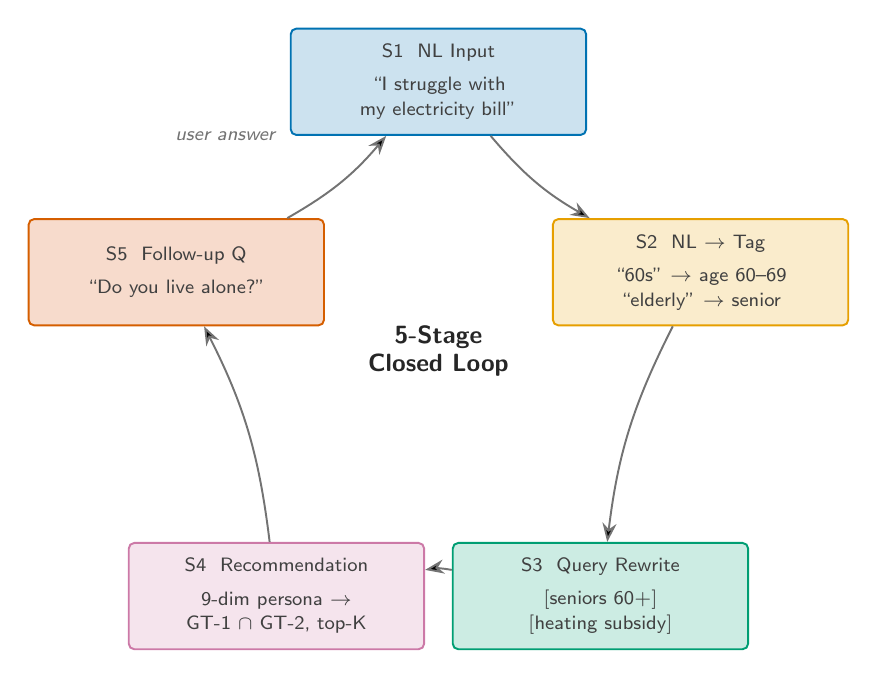
\begin{tikzpicture}[
  font=\sffamily,
  >={Stealth[length=2.4mm,width=1.8mm]},
  every node/.style={inner sep=2pt},
  stagebox/.style 2 args={
    rectangle, rounded corners=2pt,
    draw=#1, line width=0.7pt,
    fill=#2,
    align=center,
    text width=3.4cm, minimum height=1.35cm,
    inner sep=5pt,
    font=\sffamily\fontsize{7.5}{9.0}\selectfont, text=black!75,
  },
  % Match Fig 1/2 typography: bold black titles (color cue is the box border).
  stitle/.style={font=\sffamily\bfseries\fontsize{9.0}{11}\selectfont},
  sbody/.style={font=\sffamily\fontsize{7.5}{9.0}\selectfont, text=black!75,
    align=center},
  loopArr/.style={->, draw=black!55, line width=0.7pt},
]

% Pentagon centers at radius R, starting top (S1) clockwise.
% Angles: 90, 18, -54, -126, 162 (degrees).
\def\R{3.50}
% Compute positions (LaTeX-side polar coords).
\coordinate (C1) at ({\R*cos(90)},  {\R*sin(90)});       % S1 top
\coordinate (C2) at ({\R*cos(18)},  {\R*sin(18)});       % S2 upper-right
\coordinate (C3) at ({\R*cos(-54)}, {\R*sin(-54)-0.20}); % S3 lower-right
\coordinate (C4) at ({\R*cos(-126)},{\R*sin(-126)-0.20});% S4 lower-left
\coordinate (C5) at ({\R*cos(162)}, {\R*sin(162)});      % S5 upper-left

% --- 5 stage boxes: bold black title + body, centered (horiz & vert) in box ---
\node[stagebox={cbBlue}{fillBlue}] (S1) at (C1)
  {\stg{S1\ \ NL Input}\\[3pt] ``I struggle with my electricity bill''};
\node[stagebox={cbOrange}{fillOrange}] (S2) at (C2)
  {\stg{S2\ \ NL $\to$ Tag}\\[3pt] ``60s'' $\to$ age 60--69\\``elderly'' $\to$ senior};
\node[stagebox={cbGreen}{fillGreen}] (S3) at (C3)
  {\stg{S3\ \ Query Rewrite}\\[3pt] $[$seniors 60$+]$\quad$[$heating subsidy$]$};
\node[stagebox={cbPurple}{fillPurple}] (S4) at (C4)
  {\stg{S4\ \ Recommendation}\\[3pt] 9-dim persona $\to$ GT-1 $\cap$ GT-2, top-K};
\node[stagebox={cbRed}{fillRed}] (S5) at (C5)
  {\stg{S5\ \ Follow-up Q}\\[3pt] ``Do you live alone?''};

% Curved arrows along the pentagon (S1->S2->S3->S4->S5->S1).
% bend right gives a clockwise gentle curve.
\draw[loopArr, bend right=10] (S1) edge (S2);
\draw[loopArr, bend right=10] (S2) edge (S3);
\draw[loopArr, bend right=10] (S3) edge (S4);
\draw[loopArr, bend right=10] (S4) edge (S5);
\draw[loopArr, bend right=10] (S5) edge (S1);

% Center label
\node[font=\sffamily\bfseries\fontsize{9.5}{11}\selectfont, text=black!85]
  at (0, 0.25) {5-Stage};
\node[font=\sffamily\bfseries\fontsize{9.5}{11}\selectfont, text=black!85]
  at (0,-0.10) {Closed Loop};

% "user answer" hint on the S5 -> S1 return arc (between S5 and S1 mid-arc)
\node[font=\sffamily\itshape\fontsize{6.6}{8}\selectfont, text=black!55]
  at ($ (S5.north)!0.5!(S1.west) + (-0.10,0.18) $) {user answer};

\end{tikzpicture}
\end{document}
